\begin{frame}{Processus}

\begin{columns}
  \column{0.38\linewidth}
\begin{figure}
    \centering
    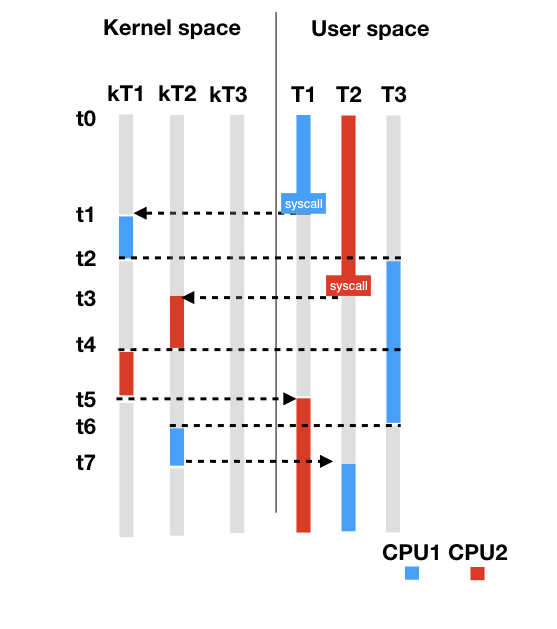
\includegraphics[width=\textwidth]{slides/images/scheduling.jpg}
\end{figure}

\column{0.58\linewidth}

\subtt{État d'un processus}

 \begin{itemize}[label=$-$]
     \item Registres processeur
     \item Table des descripteurs fichiers
     \item Répertoire courant
     \item Variables d'environnement
 \end{itemize}
\end{columns}

\end{frame}

\begin{frame}{\texttt{fork}}

    fonction Unix.fork : unit -> int

    crée un nouveau process avec le même état
\end{frame}

\begin{frame}[fragile]{Boucle de lecture avec gestion des erreurs}
\begin{lstlisting}
    let minishell () =
       try
         while true do
           (* Lecture de l'entree standard *)
           let cmd = input_line Stdin.stdin in
           match Unix.fork () with
             | 0 -> (* Processus fils *)
               let cmd = parse cmd_line in
               exec_cmd cmd;
               exit 0
             | pid_son -> (* Processus père *)
               let pid, status = Unix.wait() in
               (* Affiche le status de sortie du fils *)
                print_status "Program" status
         done
       with End_of_file -> ()

    let () = Unix.handle_unix_error minishell ()
\end{lstlisting}
\end{frame}
\begin{frame}{Encore plus de fonctionnalités}
  \begin{itemize}[label=\small\ding{114}]
  \item des commandes externes (pas implémenté en OCaml (!!))
  \item des redirections (\texttt{<} \texttt{>})
  \item des tubes  (\texttt{|})
  \item les combinateurs AND et OR  (\texttt{$\&\&$} et \texttt{$||$})
  \end{itemize}
  \todo{capture shell}
\end{frame}

\begin{frame}[fragile]{AST évolué}
    \begin{itemize}[leftmargin=-10pt]
         \item
        \begin{lstlisting}
            type cmd_kind =
                | Internal of command  (* les commandes precedentes *)
                | External of string list  (* la triche avec execvp *)
                | Cd of string
            type redirection =
                | In of string (* > *)
                | Out of string (* < *)
            type t =
                | Command of cmd_kind * redirection list
                | Pipe of t * t (* | *)
                | And of t * t  (* && *)
                | Or of t * t   (* || *)
            val execute : t -> unit
        \end{lstlisting}
    \end{itemize}
\end{frame}

\begin{frame}[fragile]{Nouvelle boucle de lecture}
\begin{lstlisting}
let minishell () =
 try
     prompt None;
     while true do
       let cmd = input_line Stdlib.stdin in
       try
         let cmd = Ast.parse cmd in
         let code = interprete cmd in
         prompt (Some code)
       with
       | Parser.Parsing_error err -> Parser.print_error err
       | Parser.Empty_line -> ()
     done
   with End_of_file -> ()
\end{lstlisting}
\end{frame}

\begin{frame}{\texttt{cd}}

\end{frame}

\begin{frame}{\texttt{fork}}

\end{frame}
